\subsubsection{Description}

During the energy bombardment phase, the layer is being bombarded by multiple particles. When a cell is hit by a particle, the impact cell and the ones near it receive some of the particle's energy and the further a neighboring cell is to the impact cell, the less energy it receives.

When a cell is far enough from the point of impact of the particle, to the point where the energy it receives is below a certain threshold (which depends on the material), the value of the energy received is counted as negligible and it is not added to the cell.

\subsubsection{Parallel version implementation}

Depending on the particle, there could be time saved by only updating the values of certain cells. Since the bigger the distance from the cell of impact, the lower the energy on subsequent cells, after a certain point it becomes unnecessary to calculate the energy that the subsequent cells receive, because if the current cell is below the threshold, the next cell will also be, because the energy received can only go lower.

\begin{figure}[h]
    \centering
    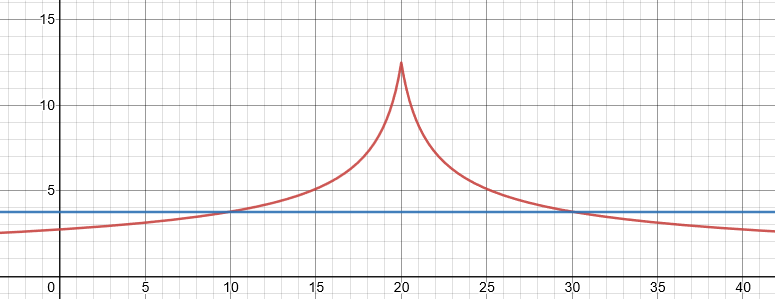
\includegraphics[scale=0.4]{images/Threshold.png}
    \caption{With the layer being the x axis and energy being the y axis in this figure, only the x positions where the red function (energy received by the particle) is above the blue line (the threshold) are relevant for updating}
    \label{fig:my_label}
\end{figure}



From these equations, we can calculate the positions of the limits of the layer, inside of which the energy received by each cell is above the threshold.


\begin{equation*}
distance =  \lvert pos - k\rvert+1\\  

attenuation = \sqrt{distance}\\

 energy_k = energy / layer\_size / attenuation\\
 
energy_k \geq threshold/layer\_size\\

threshold/layer size \leq energy / layer\_size / attenuation\\

\iff attenuation \leq  energy/threshold\\

\iff distance\leq (energy/threshold)^2 \\

\iff k = pos + (energy/threshold)^2 -1 \lor k = pos - (energy/threshold)^2 - 1\\

\end{equation*}

So instead of trying to update the whole layer, and only updating the relevant cells, it now only updates the relevant cells from k\textsubscript{min} to k\textsubscript{max} , which can save considerable time when the the amount of cells in the layer and/or the threshold are high.

The second step is to simply divide the resulting layer for each thread using OMP and update it. Since the update function has no dependencies among cells there will never be any concurrency issue among them.

\begin{figure}[h]
    \centering
    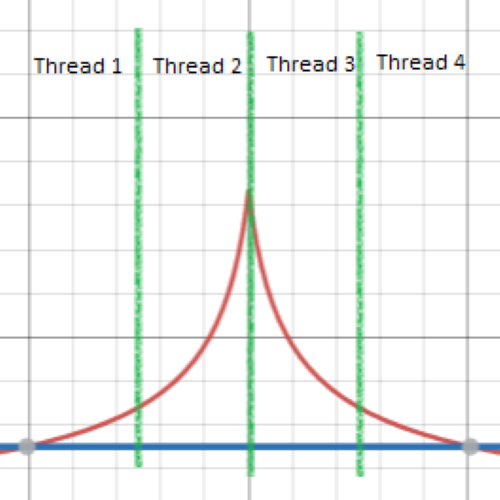
\includegraphics[scale=0.4]{images/Thread_separation.png}
    \caption{The easiest way to quickly compute the energy on the relevant part of the layer is to divide the relevant part equally for each thread}
    \label{fig:my_label}
\end{figure}

Another approach could have been for instead of dividing the layer for each thread, dividing the storm particles for each thread. This would make it so the layer is shared among threads, and there will be an output dependency when the threads update the same cell. To bypass this issue, there's the possibility of updating the cells atomically, wasting the efficiency of concurrency, or having each thread work on its own layer, and adding them all at the end, which would drastically increase space used and also increasing time by adding them all, compared to the chosen solution.



